\section{Results}

% \begin{figure*}
%  \subfigure[EHP vs. Light]{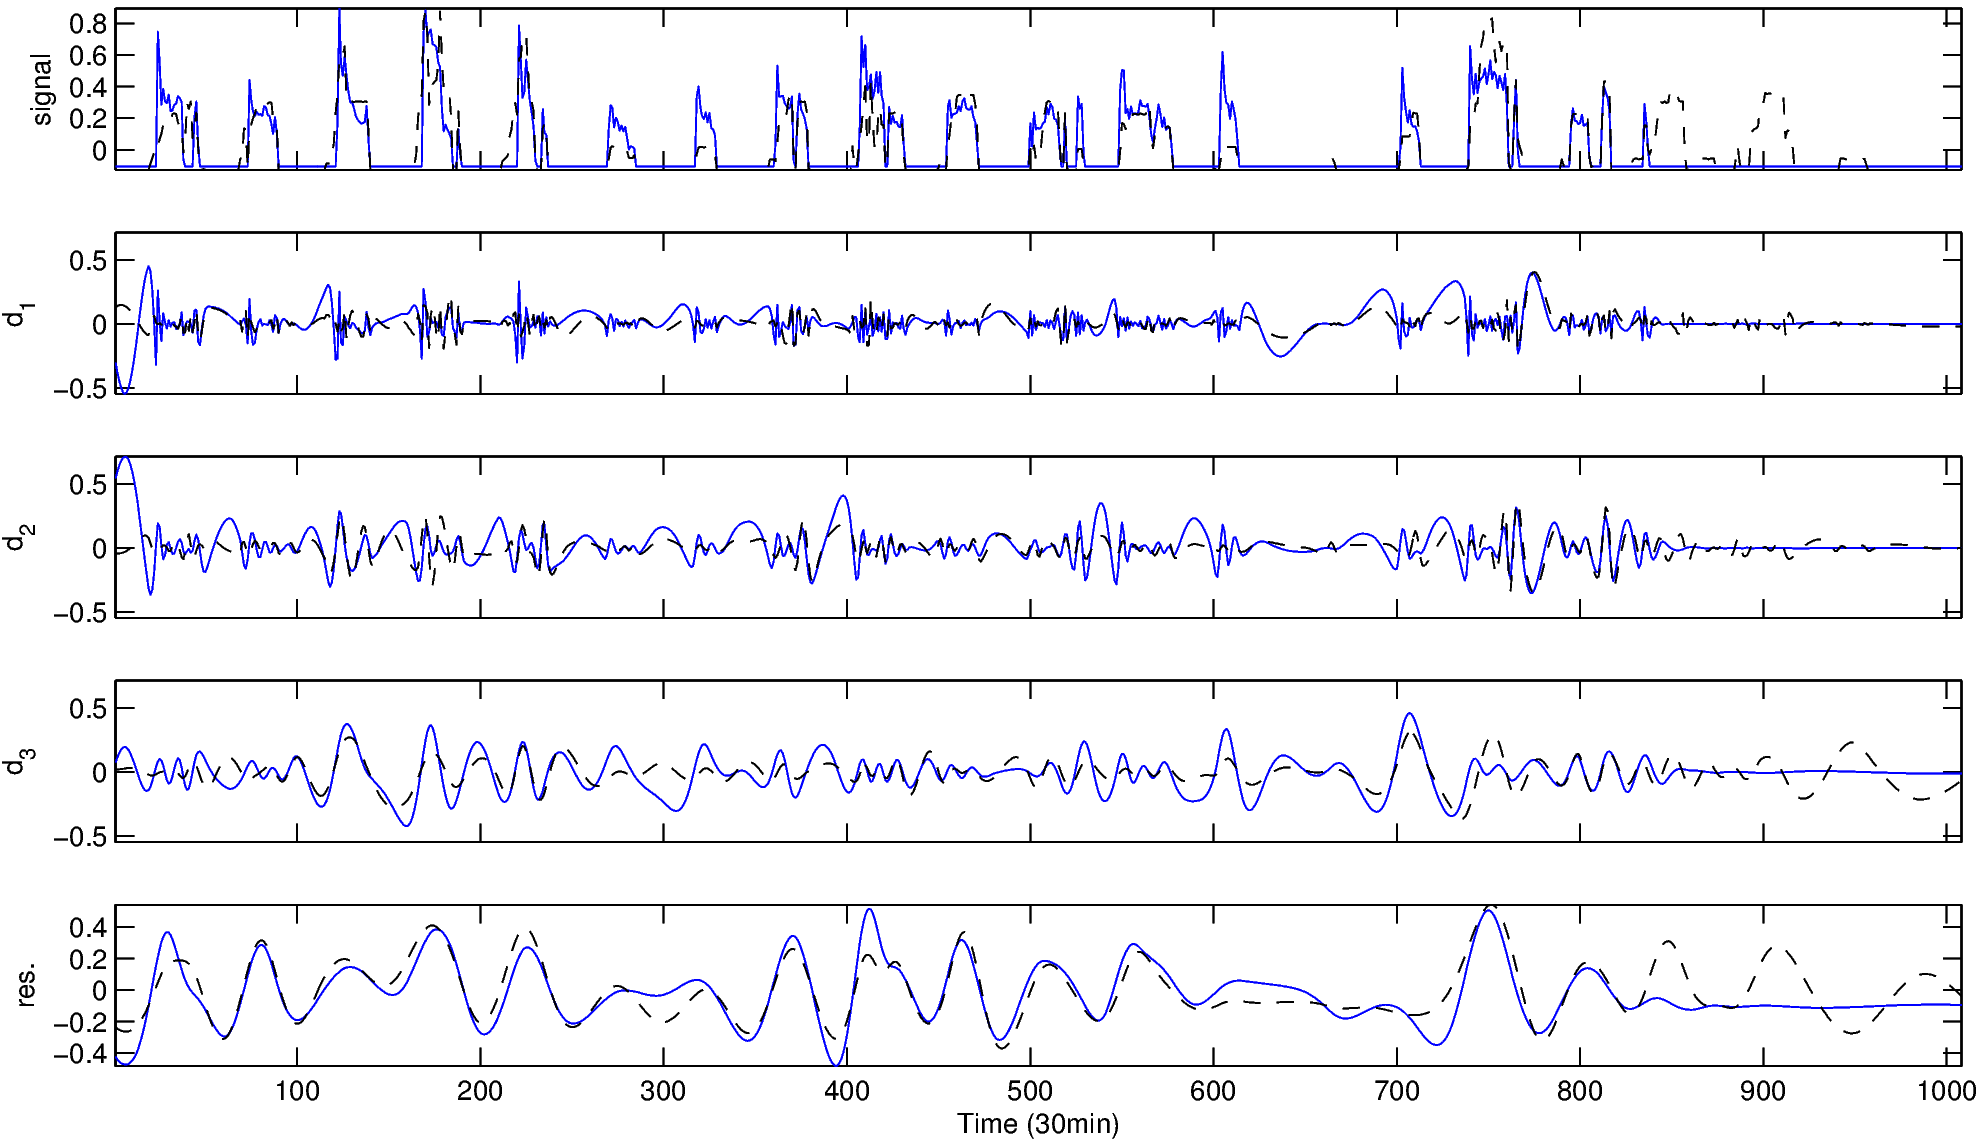
\includegraphics[width=\textwidth]{img/emd_25_26}}
%  \subfigure[EHP vs. GHP]{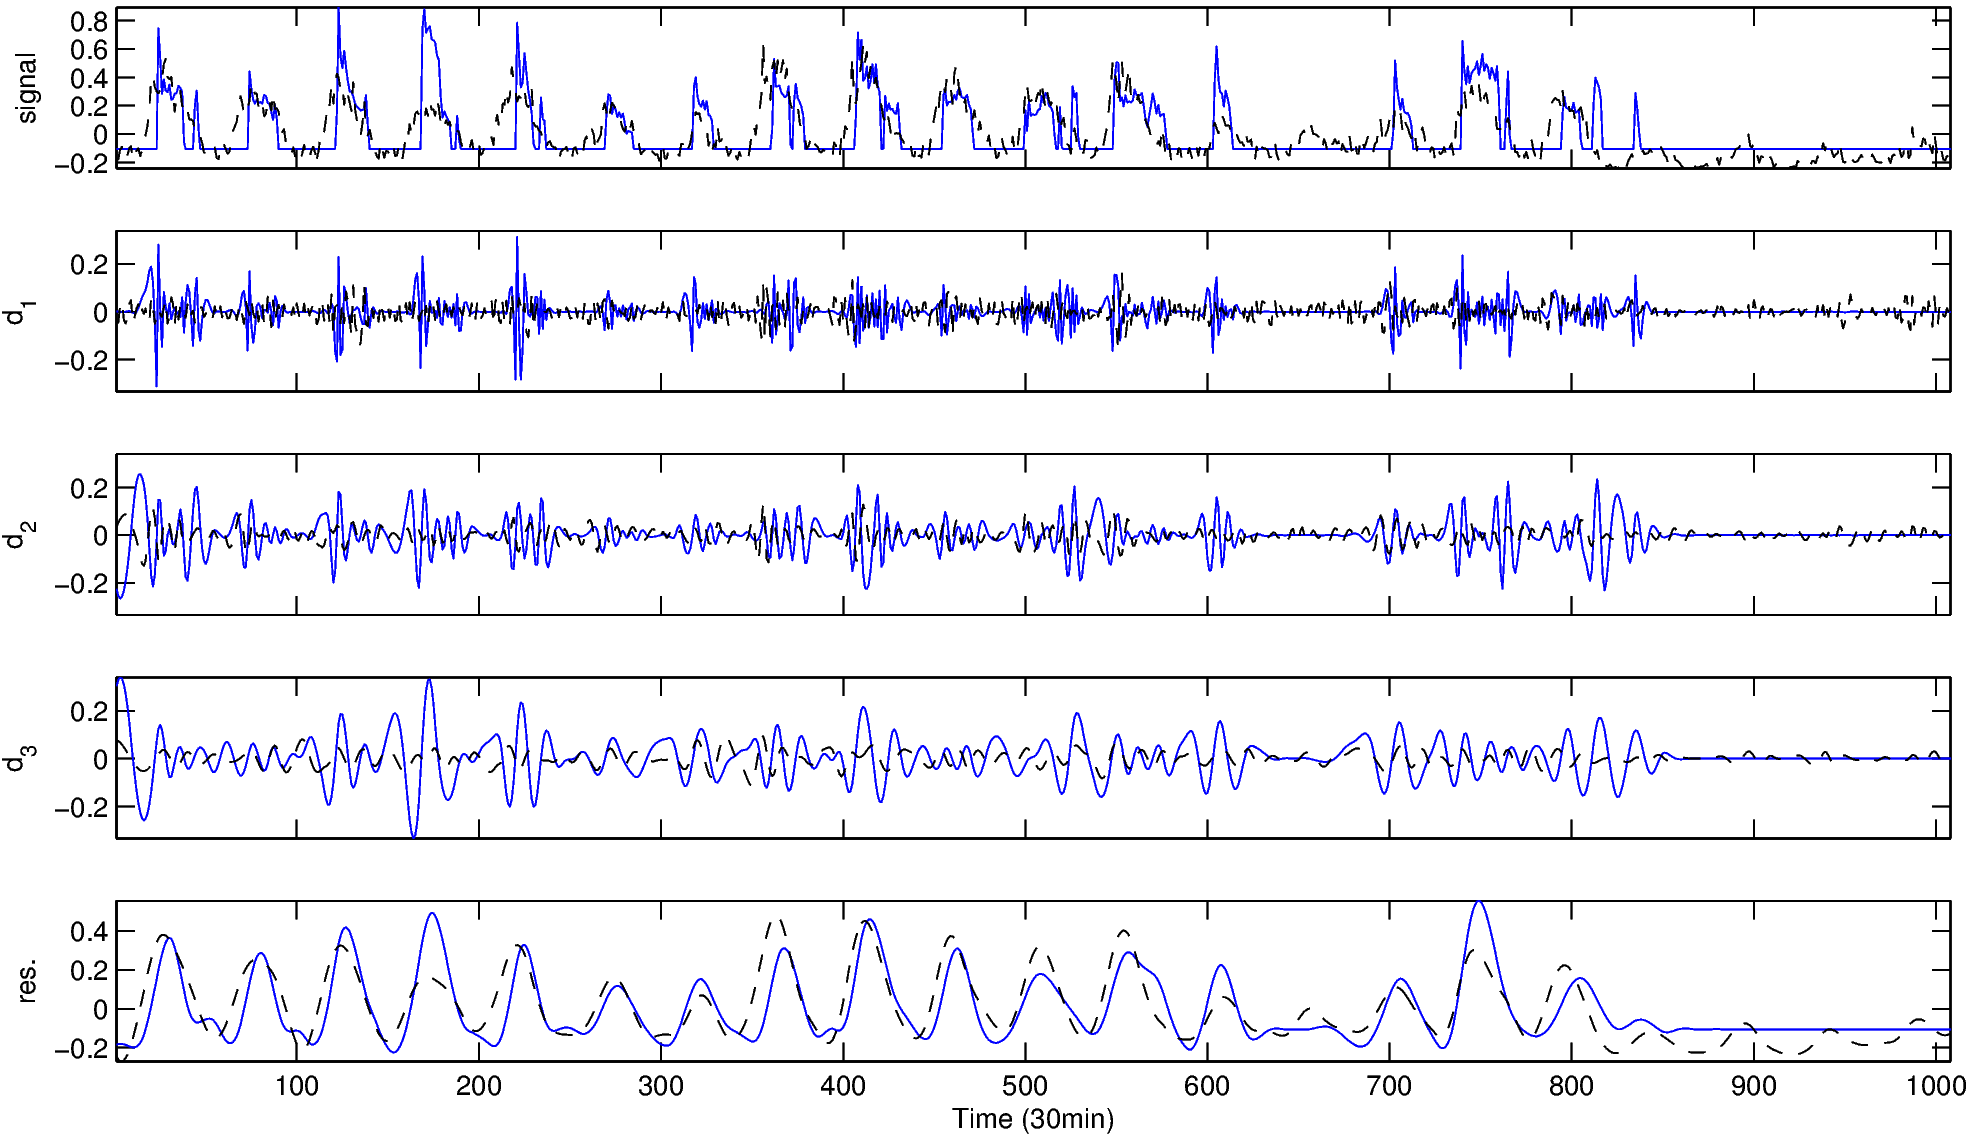
\includegraphics[width=\textwidth]{img/emd_25_41}}
%  \caption{Empirical Mode Decomposition}
%  \label{fig:emd}
% \end{figure*}



This section emphasizes the advantages of EMD to effectively uncover correlated sensor traces.
First, we demonstrate the benefit of EMD with a simple example, the three sensors presented in Section \ref{problem}.
Second, we validate the proposed methodology using a large dataset (674 sensors) and highlight the ability of EMD to uncover the spatial correlations of the sensors.

\subsection{Example with 3 sensors}
Lets consider the simple example of Section \ref{problem} where we would like to know if the EHP trace is correlated with the two other traces; the light trace and the GHP trace.
Using the raw traces, the correlation coefficients $0.7715$ and $0.6370$ corresponding respectively to the light and GHP trace suggest that both traces are correlated to the EHP trace.
% As stated in previous section this result is biased by the strong daily pattern shared by these three traces.
As stated in previous section this result is misleading, as the weather trend dominates the calculation.
%We emphasize that extracting the daily pattern of the data using EMD permits a more detailed analysis of these traces.
Figure \ref{fig:emd} and Figure \ref{fig:emd2} show the EMD decomposition of the three traces.
%Notice that the EMD process has been voluntary stopped once the daily pattern has been uncovered.
For each trace, EMD has retrieved three IMFs that highlight the higher frequencies of the traces.

Figure~\ref{fig:emd} show the raw signal (top) and EMD output IMFs and residual as well as the 
correlation coefficients calculated on the IMFs for the EHP and
light traces.  The correlation coefficients are $0.43909$, $0.49344$ and $0.63469$ corresponding to the IMF1, 
IMF2, and IMF3, respectively.  Notice the highly correlated high-frequency IMF results.
Figure~\ref{fig:emd2} shows the similar information, but for the EHP and GHP.
The correlation coefficients for the EHP and GHP IMFs suggest that the two traces are independent in their 
high-frequency IMF components.
EMD allows us to meaningfully discriminate between traces, indicating the underlying independence in the intrinsic
behavior of the two heat pumps.  It also suggest that the EHP and light are more intrinsically related
to one another.  Although promising, these results must be validated across the rest of the
dataset to confirm their significance.  
% Figure \ref{fig:emd} and \ref{fig:emd2} summarize our findings.
% permits to effectively identify that the light trace is related to the EHP whereas the GHP one is not.

\subsection{Validation}
To validate the effectiveness of our approach, we analyze the same three-week time span as the
initial exercise for \emph{all} 674 sensors deployed in the building.
For each trace $S$ we compute two scores: (1) the correlation coefficient for $S$ and the EHP trace, (2) the average value of the two traces IMFs correlation coefficients.

\begin{figure}[tbh!]
\centering
 \subfigure[Raw traces correlation coefficients]{\label{fig:histo1}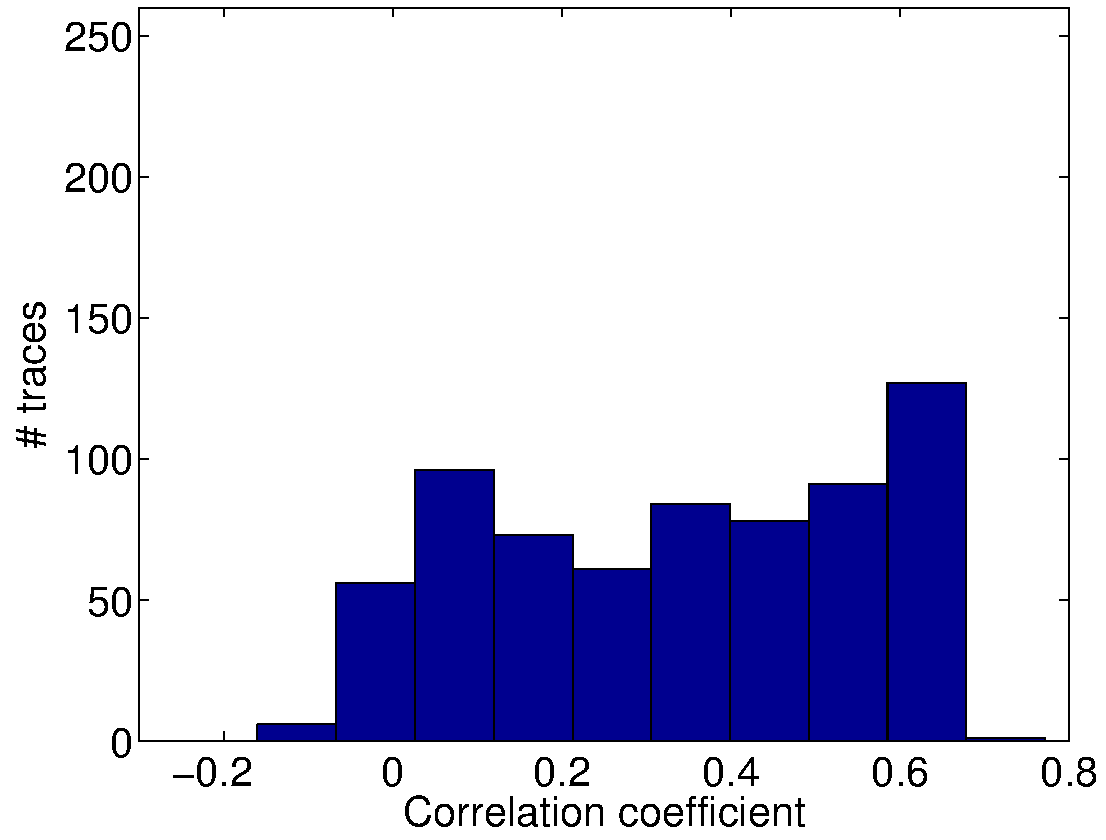
\includegraphics[width=.43\textwidth]{img/allFloors_week1_week4_corr_abs-eps-converted-to}}
 \subfigure[Average IMFs correlation coefficients]{\label{fig:histo2}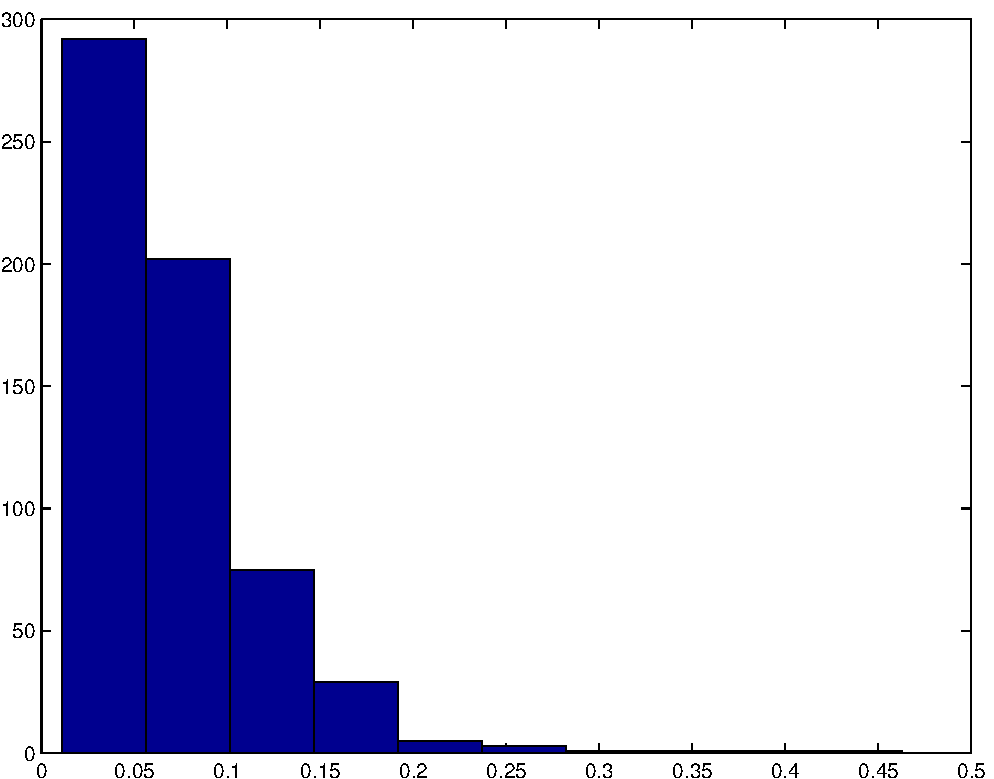
\includegraphics[width=.43\textwidth]{img/allFloors_week1_week4_emd_abs-eps-converted-to}}
 \caption{Distribution of the correlation coefficients of the raw traces and corresponding IMFs using 3 weeks of data from 674 sensors deployed on 12 Floors.}
\label{fig:histo}
\end{figure}

\begin{figure}
\centering
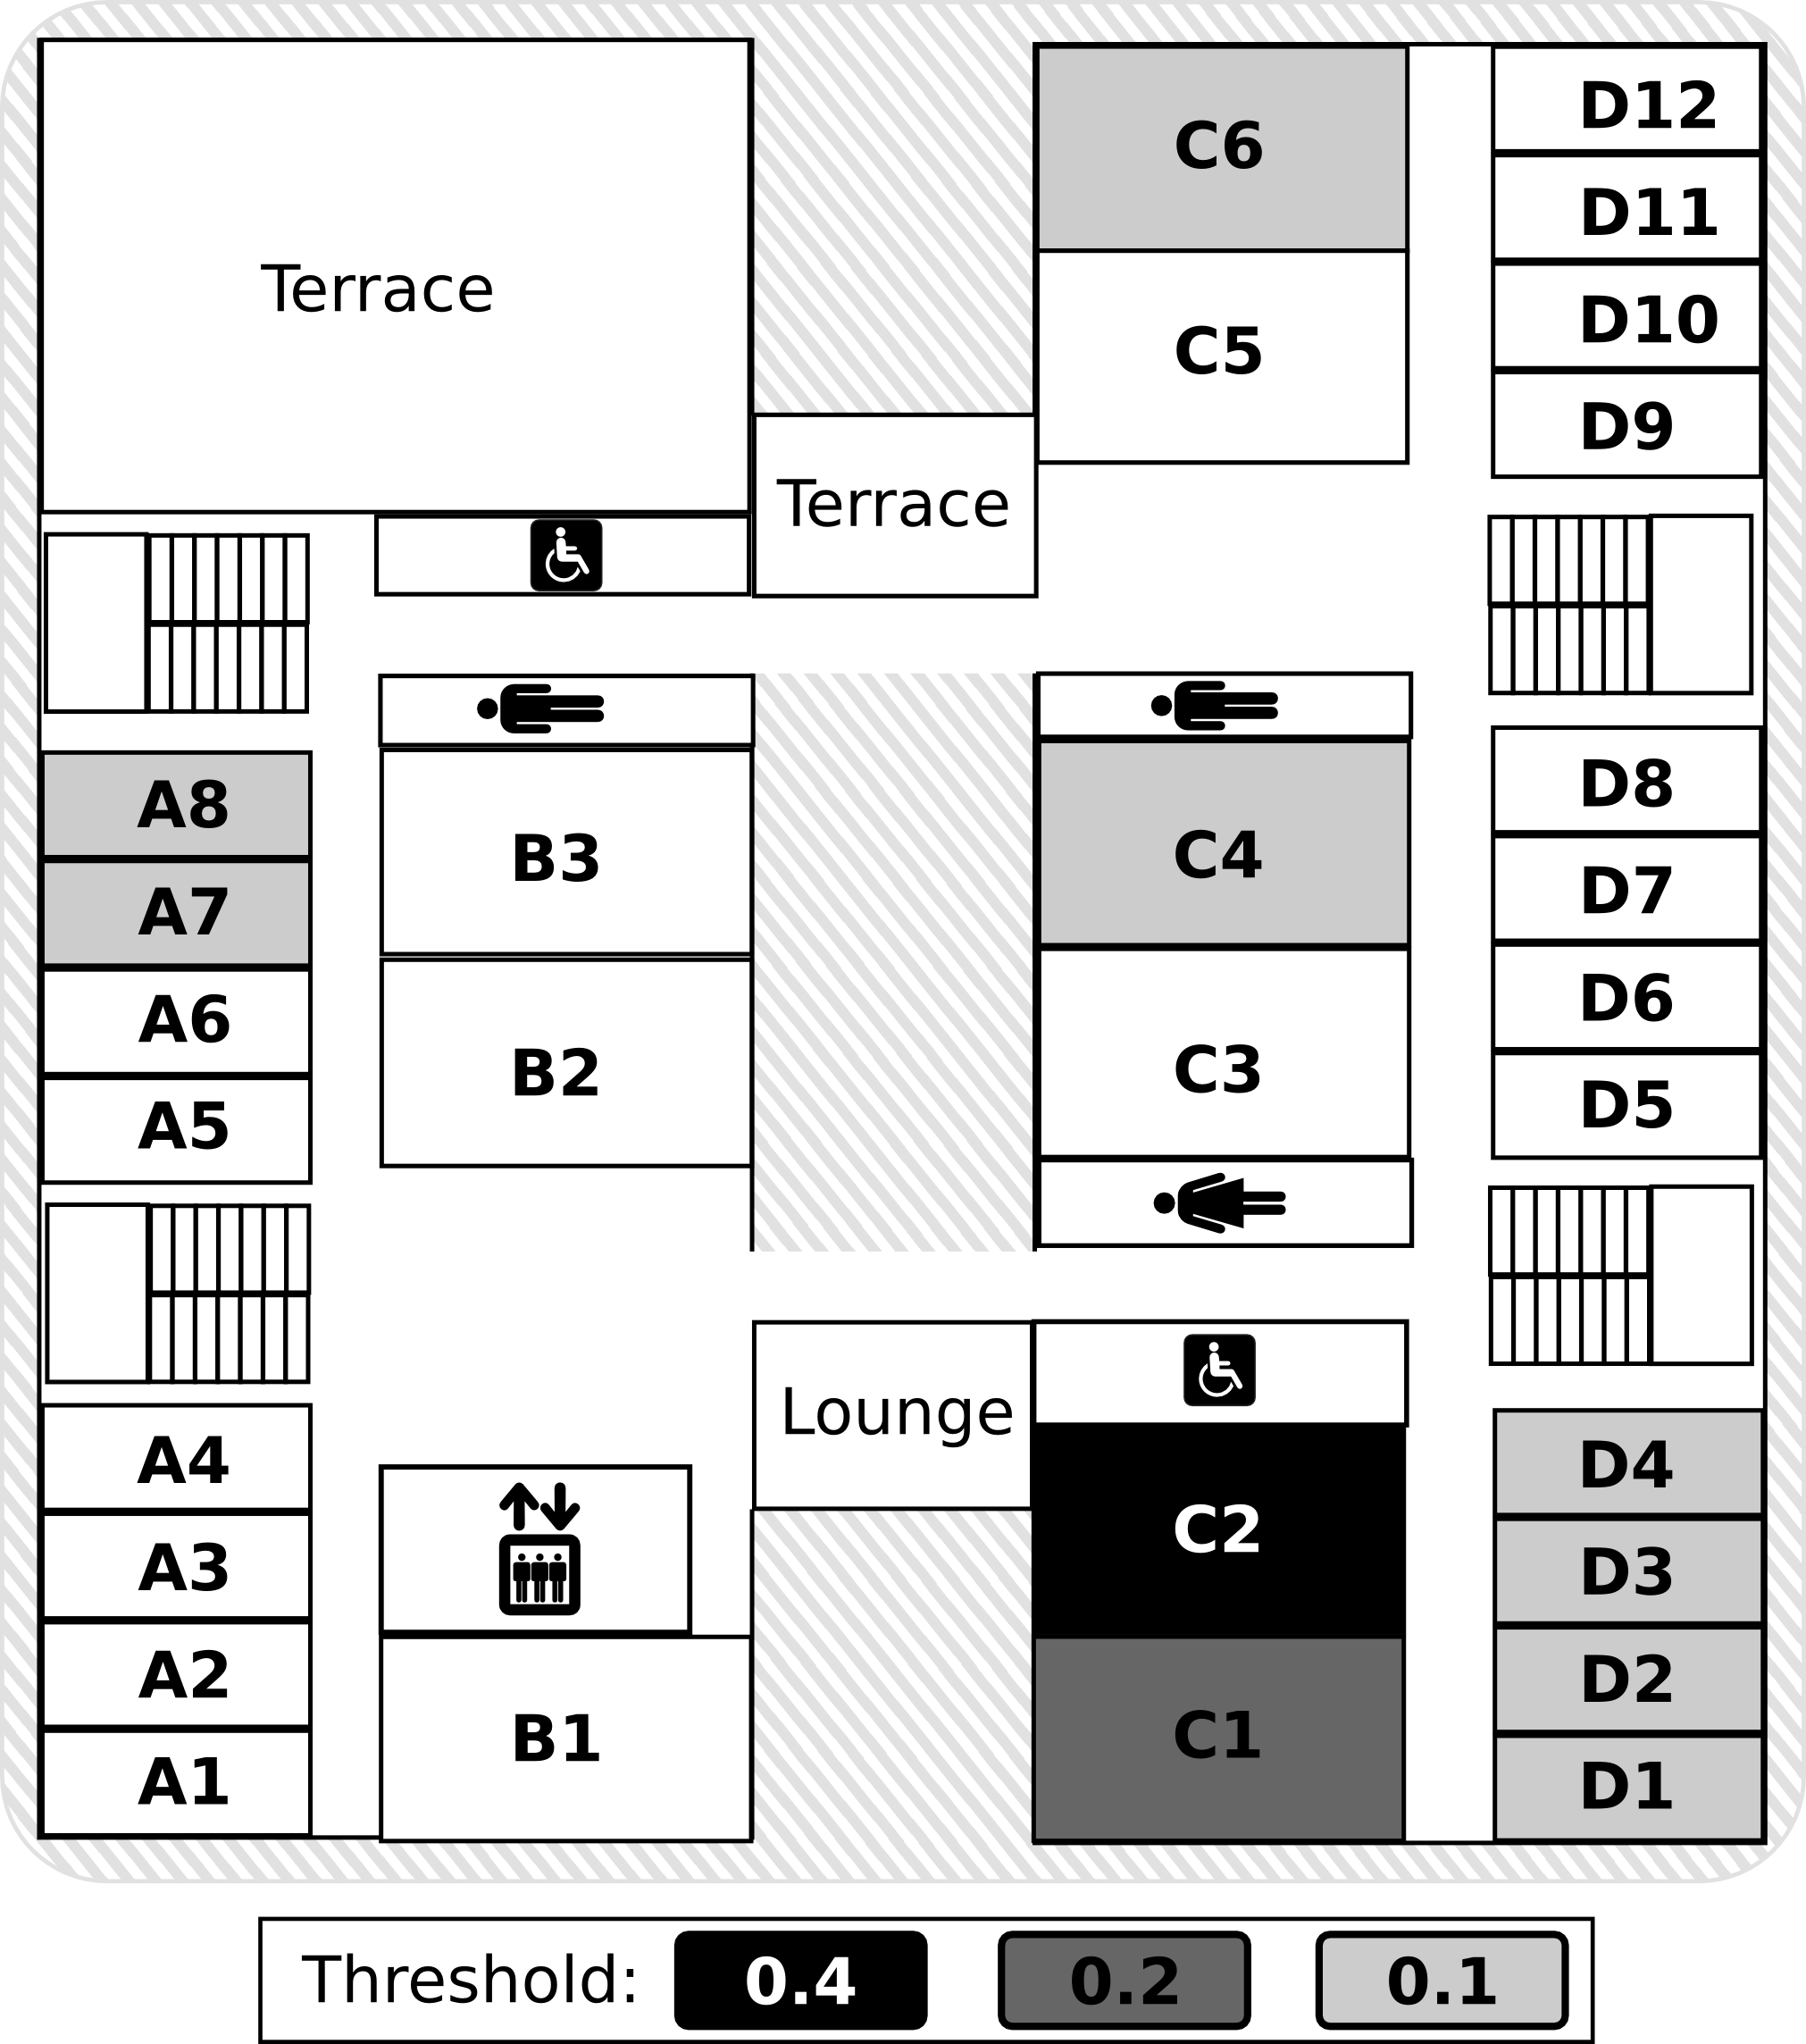
\includegraphics[width=.45\textwidth]{img/floorMap.png}
\caption{Map of the floor where the analyzed is EHP trace is measured (room $C2$). The location of the sensors identified as related by the proposed approach are highlighted.}
\label{fig:map}
\end{figure}

Figure \ref{fig:histo1} shows the distribution of the traces' correlation coefficients.  Notice
that a large fraction of the dataset is correlated with the EHP trace.
Indeed, \emph{half} the traces have a correlation coefficient higher than $0.36$.  As expected, the underlying
trend is shared by a large number of device.
Although the highest score (i.e. $0.7715$) corresponds the light in the same room that the EHP serves,
there are 118 pumps, serving all areas of the building, with a correlation higher than $0.6$.
Using only these results, it is not clear where the threshold should be set.  The distribution is close to 
uniform, making it difficult to 
know of how well your threshold discriminates against unrelated traces.
% Moreover, the distribution of the traces is almost uniform, thus, discriminating correlated traces is a laborious task.

Figure \ref{fig:histo2} shows the distribution of the average correlation coefficients for the IMFs of
each trace and the EHP.  The number of traces correlated in the high frequency IMFs is significantly smaller
than the previous results. It's clear from the distribution that only a small set of devices are
\emph{intrinsically correlated} with the EHP.  Only 10 traces out of 674 perform with a score higher than 
$0.25$. This allows us to easily rank traces in term of correlation.

Upon closer inspection of the 10 most correlated IMF traces, we find that there is a spatial relationship
between the EHP and the 10 devices.  In fact, there is a direct relationship between score and distance from
the areas served by the EHP.  Figure~\ref{fig:map} shows a map of the floor that contains the rooms served by this
EHP.  The EHP directly serves room $C2$.  We highlight rooms by the threshold setting on the IMF correlation coefficients.
When we set the threshold at $0.4$ we see that the sensors that have a correlation higher fall within room $C2$ --
the room served directly by the EHP.  As we relax the threshold, lowering it to $0.2$ and $0.1$ we see radial expansion from $C2$.  The trace with the highest score, $0.522$, is the trace corresponding to the lighting system \emph{in
the same room}.
The two highest scores for this floor (i.e. $0.316$ and $0.279$) are the light and EHP traces from next door, room $C1$.
Lower values correspond to sensors measuring activities in other rooms that have no specific relationhip to the analyzed trace.  The results show a direct relationship between IMF correlation and spatial proximity.


% Interestingly, the IMFs correlation coefficients reveal the spatial correlation of the sensors.
% Figure \ref{fig:map} is the map floor where the EHP trace is measured.
% Specifically, the EHP reports heating activity in the room $C2$.
% in the simple scenario the GHP is located in the room A5.


